\documentclass[12pt,a4paper]{article}
\usepackage[latin1]{inputenc}
\usepackage{amsmath}
\usepackage{amsfonts}
\usepackage{amssymb}
\usepackage{listings}
\usepackage{color}
\usepackage{hyperref}
\usepackage{graphicx}
\usepackage{prettyref}
\usepackage{cite}
\newrefformat{lst}{Listing \ref{#1}}
\newrefformat{list}{List \ref{#1} on page \pageref{#1}}
\definecolor{lightGray}{gray}{0.95}
\lstset{
backgroundcolor=\color{lightGray},
breaklines=true,
captionpos=b,
frame=single,
keepspaces=true,
keywordstyle=\color{blue},
language=HTML,
morekeywords={created,modified,tags,img,\$button,message},
numbers=left
}
\usepackage{float}
\newfloat{lablist}{H}{lol}
\floatname{lablist}{List}

\newcommand{\todo}[1]{{\bf TODO: #1}\\
}

\title{Analysis and documentation of a single page application based on TiddlyWiki}
\author{Christian Jurke 898872, Christian Heigele 901361}
\begin{document}
\maketitle
\tableofcontents
\textbf{Pages Min:15.5 Max:20 }
\section{Introduction 1}
\section{Decomposition of the TiddlyWiki-Architecture 6}
Traditional web applications are bound to HTTP-Concepts, including stateless requests to transfer data. In these applications a state is often emulated by the use of sessions, which need to be handled on the client and especially on the server side.
These restrictions often lead to a fragmented user experience because the user interface is rebuilt on every data transfer.
TW tries to overcome these restrictions and the resulting disadvantages by building on few but basic concepts which loosen the coupling of HTTP and the actual application eliminating the need of state emulation and resulting in a wiki style single page application with the ability to run in an offline environment.
\subsection{Architecture of the single page application TiddlyWiki 3}
TW builds on some basic concepts. First, TW should not be perceived as a dynamic web page like traditional server-side generated web pages. Instead TW can be perceived as an application which is written entirely in JavaScript and uses HTML5 and CSS3 to render a GUI. This way TW can be executed in any JavaScript environment, like a browser or a node.js instance, while keeping the advantages of a simple application.
One of these advantages is, that TW has no need to emulate an application state, like a traditional web application would need to do.

A second concept concerns the storage of the application data. In contrast to a traditional web application, TW doesn't store the data in an external database but simply uses native data structures already existing in JavaScript to store tiddlers, the basic (atomic) element of the TW application, in the memory. Additional core modules provide a way to persist this storage in simple HTML div elements.

Just by building on these simple and basic concepts,
\begin{itemize}
\item TW is able to store application data in a single HTML page by using div elements as data container.
\item TW is able to store application code (JavaScript) in the same single HTML page.
\item TW can be executed in any JavaScript environment like a browser.
\end{itemize}

These points already enable TW to be used as an offline-enabled single file web application.
Also, by using a server side node.js environment, TW can be used as an online web application, just by providing an additional module to persist tiddlers into plain text files and a module syncing the local data store with the node.js server.

%\todo{tiddlers, modules, plugins}
%\todo{in memory datastore (Wiki) and filter as query language}
To understand the architecture of TW, the first important thing to understand is that anything is a tiddler.
Even the application logic is stored in tiddlers that are marked as "application/javascript".
These tiddlers, which contain application logic, are called modules and a CommonJS compatible module system is responsible for assembling the individual modules into the TW application.
The result is a tree representing the whole TW application containing module tiddlers, data tiddlers and some JavaScript functions and objects.

\subsubsection*{Boot Kernel}
Only a small part of the TW is not managed as tiddlers, the boot kernel.
The boot kernel is the first thing running, when the application is started and it puts some initial objects and functions into the application tree, which are needed to load and manage tiddlers.
After the boot kernel built this initial application tree, the remaining parts of the application can be loaded as module tiddlers.
Beside some utility functions the most important object that is contributed by the boot kernel is "\$tw.wiki", consisting of JavaScript structures and functions that are used to store and manage the loaded tiddlers.
Among other things this store can be used to add new tiddlers, remove tiddlers and retrieve tiddlers by name.

%\todo{data persistence (saver and deserializer)}
\subsubsection*{Data Persistence}
The next important part of the application are deserializers. Deserializers are responsible to load tiddlers from various sources. One of the deserializers provided by the boot kernel for example can load new tiddlers from the current DOM tree.
The counter part of the deserializers are savers and syncadapters.
Both are used to persist the changes made to the store but they work in slightly different ways.
A syncadapter registers at the store for changes.
Now when a tiddler is changed and these changes are written to the store, the syncadapter is triggered and persists the new changes, for each tiddler individually.
If no syncadapter is available a saver can be used to persist new changes.
A saver does not register to change events and so it does not persist each tiddler, when it is changed.
A saver is used to save the complete store or the complete TW for that matter at once. After a user made changes to some tiddlers, this method can be used to download the current state of the store as a completely new TW application.

%\todo{interpreting wiki text (parser)}
%\todo{ui (widgets, dom tree)}
%\todo{sync data store with ui - selective update}
\subsubsection*{UI - WikiText and Widgets}
Following the "anything is a tiddler" concept, even the UI consists of tiddlers.
This is possible because tiddlers can not only contain plain text or JavaScript (modules) but the also can contain a special markup text called WikiText.
By using WikiText the user can put markup elements like tables or images in a tiddler.
To provide some more sophisticated UI elements, WikiText can also contain special widgets like text input fields,
checkboxes, dynamic lists etc.
In most cases, these widgets are used to directly modify or represent the information contained in other tiddlers.
If a tiddler is changed and this change should reflect in the UI e.g. a widget, a process called selective update takes place. Selective updating means when a tiddler or a set of tiddlers changes, each widget is asked, if changes to this tiddlers would affect its appearance. If so, the respective widget is re-rendered otherwise it remains unchanged.

\subsubsection*{Modularization}
The whole application is basically built from three parts. At first, the boot kernel provides the basic functionality to handle tiddlers. The second part are tiddlers representing core functionality. These are for example modules which extend the store by more sophisticated functions, UI tiddlers and widget modules, a WikiText parser, sophisticated deserializers, savers, syncadapters, etc.
At this stage the application can be extended by plug-ins. Consequently, a plug-in is a single tiddler which itself contains multiple tiddlers, forming the plug-in. Each of this tiddler might be a module providing new functionality (i.e. a module tiddler marked with "module-type: saver" can extend the application with new methods of saving the current wiki state.).
Also, a tiddler contained in a plug-in can supersede" an existing tiddler and take its place.

By managing nearly every part of the application as tiddlers, the application is only needed to provide some basic functionality to manage the individual tiddlers, load and persist them, render them to HTML output and provide a way to register for the changes made to tiddlers.
This way the whole wiki application can be build from these simple concepts.
Plug-ins can be used to add new functionality to the existing modules or even to replace individual tiddlers/modules,
enabling developers to build whole new applications on the TW base system.

\begin{figure}[hbtp]
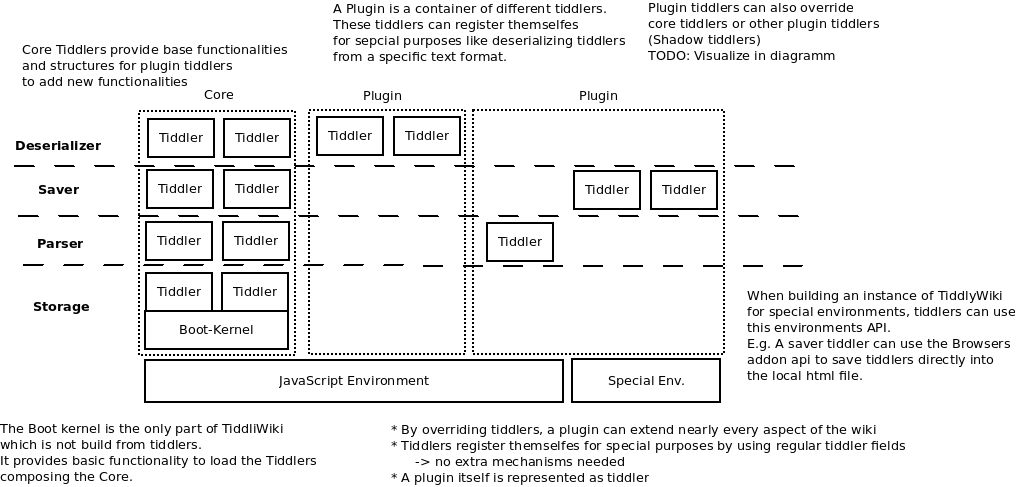
\includegraphics[scale=0.4]{images/overview.png}
\caption{Decomposition of TW}
\end{figure}
\newpage
\subsection{Tiddler as the key element 1}
%\todo{What are the parts of a tiddler - pretty much done}
%\todo{what can a tiddler be - plain text, module, image, container for tiddlers(plugin), ui-element}
%\todo{what can i do with tiddlers? - tags, filter-language, widgets modify or represent tiddlers/listoftiddlers}
%\todo{example of the concepts power: drag and drop functionality - By providing the functionality to drag and drop a tiddler from one browser to another, we can transfer anything from one tw-instance to another, including plain text, images, new modules like widgets or savers, and even a whole plug-in can be added to an existing TW instance just by draggin and dropping}

A tiddler is the smallest unit of the TiddlyWiki system. It can contain any data like plain text, WikiText markup, JavaScript code (module tiddler), JSON structures\footnote{JSON structures might even contain additional tiddlers. Plug-ins are implemented this way to pack multiple tiddlers in a single plug-in tiddler.}, images in SVG format or even binary images encoded with base64.
Internally Tiddlers are immutable (are they?) objects containing a bunch of key:value pairs called fields. The only required field of a tiddler is the title field. The Standard fields of a tiddler are listed below. Nearly everything in TiddlyWiki is loaded as tiddlers. Plugins for example are a bunch of tiddlers that are distributed as a single JSON tiddler. The only exception is the boot kernel which isn't a tiddler.
\begin{lablist}
\caption{Custom fields of a tiddler div}
\label{list:TiddlerFields}
\begin{description}
\item[created] Timestamp number of milliseconds since 01.01.1970.
\item[modified] Timestamp number of milliseconds since 01.01.1970.
\item[tags] list of tags seperated by whitespace. Tags which contain whitespaces are wrapped by [[ ]], e.g. [[example Tag]].
\item[type] Type of the Tiddler, e.g. text/plain or text/vnd.tiddlywiki .
\item[title] Title of the Tiddler
\item[list] An ordered list of tiddler titles associated with a tiddler
\end{description}
\end{lablist}

Tiddlers are used across multiple levels. Meaning a developer uses tiddlers as the basic element containing application code, configuration values and even as a form of variable to build up the wiki application.
On a different level, a tiddler is also the basic unit of work for the wiki user, e.g. the individual wiki pages are implemented as tiddler.
This makes sense for multiple reasons:
Because the UI of TW is build from tiddlers, the wiki user is able to edit the interface of his own TW just by editing a wiki page.
For example to add a list of tiddler links to the sidebar, the user just needs to create a new wiki page (in fact a tiddler), put the links into this page and tag this tiddler with "\$:/tags/SideBar".
This way the user can customize his work environment just by using mechanism he already uses to manage his wiki pages.
Tiddlers consist of fields. When using a tiddler as wiki page, the user can use these fields to store meta information, like tags.
Because fields for metadata and especially tags are an easy way for the user to organize his wiki pages, TW provides a special filter mechanism to choose tiddlers using their metadata.
A filter string like "[tag[learncard]topic[math]!tag[successful]]" would filter all tiddlers tagged with "learncard", with the value "math" in the topic-field and are not tagged with "successful".
A user could use this filter together with the "\textless\$list\textgreater" widget to display a list of all math learncards which are not yet answered successfully in a wiki page.
And because a wiki page is nothing but a tiddler, just by tagging this tiddler with "\$:/tags/SideBar", the user gets a permanent list of learncards to be done in the sidebar of his TW application.

Another example which shows how the "anything is a tiddler" concept leads to an environment where a single feature brings great benefit is the drag and drop feature.
HTML5 standard comes with a native drag and drop feature. TW uses this feature and makes it possible to drag and drop a tiddler from one instance to another.
And because anything is a tiddler, this brings the ability to drag and drop individual wiki pages, JavaScript modules, UI components and whole plug-ins between TW instances.

\subsection{The WikiText concept 1}
The WikiText is a markup language, created especially for the requirements of the TiddlyWiki application. It is based on Markdown\footnote{\url{http://daringfireball.net/projects/markdown/}}, but extended with some TiddlyWiki specific features.  On one hand its a text-to-HTML conversion language and on the other hand its used to provide the interactive features of TiddlyWiki. The aim of this language is to allow the user of the software to focus on the writing.\cite{TIDD:WIKITEXT} The WikiText is used to format Tiddlers within the TiddlyWiki application. The tags of the WikiText syntax can be used within the standard text input field. 
During the saving process these tags renders to HTML elements for example:
\begin{lstlisting}[caption={Example use of WikiText},label=lst:wikitext]
WikiText:--- 
Renders as:
HTML:<hr>
WikiText:[img[http://tiddlywiki.com/favicon.ico]]
Renders as: 
HTML:<img src="http://tiddlywiki.com/favicon.ico">
\end{lstlisting}
Furthermore the WikiText is used to access the widgets which are integrated in the application.These widgets are used to enhance the the WikiText with a rich functionality. Widgets are based on the HTML-Syntax but always starts with a \$.
\begin{lstlisting}[caption={Example use of widgets within WikiText},label=lst:widgets]
WikiText:
<$button message="tw-close-tiddler">Close Me!</$button> 
\end{lstlisting}
\newpage
\section{Bootstrap-Process 2-3}
\subsection{The Heart of TiddlyWiki (Boot-Kernel) 1 - 1.5}
The boot-kernel is responsible for creating a barbone TW environment. It is running under Node.js or in a HTML5 Browser. The Bootkernel just loads enough functionality to load the modules containing the main logic of the application. This boot-kernel contains a few helper methods, the module mechanism as well as the function to create a tiddler and manage them. The boot-kernel also creates the barbone wiki store, which holds all the information of the wiki during the runtime. After creating the store, the boot-kernel is in charge of decrypting the encrypted tiddlers and extracting all the tiddlers e.g. the core module tiddlers embedded in the DOM structure of the HTML file. Furthermore the boot kernel offers the functionality to load tiddlers from a file, when you run TW with Node.js. All other functionality which is not a part of the boot kernel is added dynamically by modules and plugins. The boot kernel is able to load the core plugins and perform the startup plugins. The core contains the startup modules shown in the picture below.
\begin{figure}[hbtp]
\caption{Core Startup Modules}
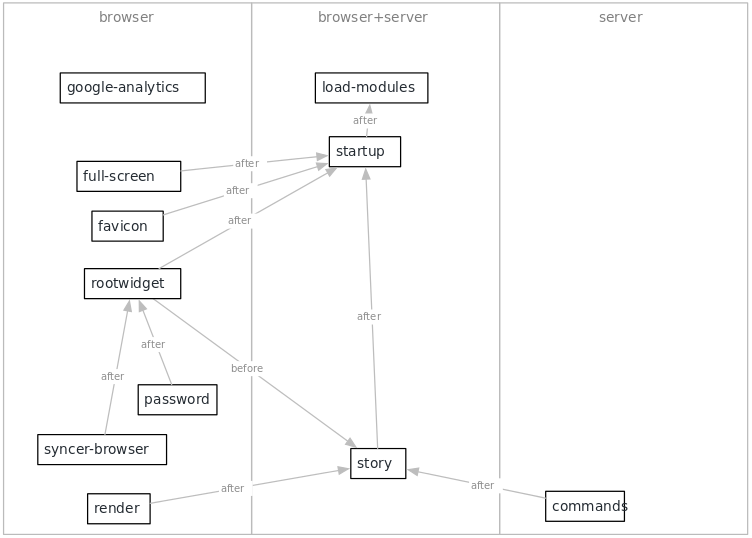
\includegraphics[scale=0.5]{images/index.png}
\end{figure}

\newpage
\subsection{Timeline of the startup Process 1 - 1.5}
This section shows a quick and short overview over the startup process of TW, from the first step of the boot mechanism until the loading of the different startup modules. The image shown below (\prettyref{fig:start}) shall point out the main parts of this startup-process.
\begin{figure}[hbtp]
\caption{Startup-Process}
\label{fig:start}
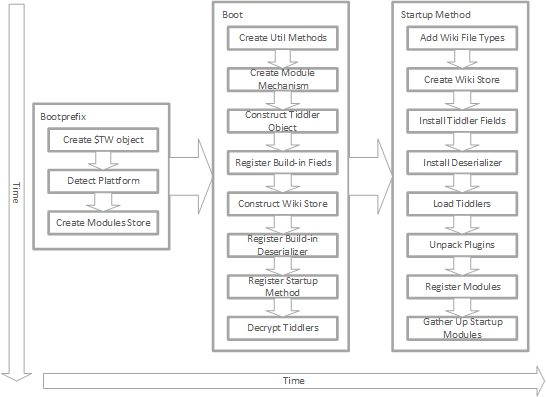
\includegraphics[scale=1]{images/StartupTimeline.png}
\end{figure}
\section{The Plugin and Module concept 4-5}
Beside the boot kernel, TW is completely build from modules.
After a short introduction on modules and plug-ins in the context of TW and explaining how they are organized and managed,
the following sections will show what type of modules a developer can build and how they hook into the TW architecture.
The last section shows the procedure of building an plug-in.
This can be used as a tutorial for building your own plug-ins and will show how an advanced user can create solutions for his own use cases only by using the tiddler model and the WikiText markup language.

\subsection{Introduction to the Module- and Plugin-Concept 1}
%\todo{building on the boot-kernel...}
%\todo{what is a module, how is a module used, included?}
%\todo{commonjs, moduletypes (global, blah, etc)}
%\todo{Plug-ins, what is a plugin, shadow tiddler}
After the boot kernel provides the functions used to load tiddlers, the rest of the TW application is loaded as modules.
A module is a tiddler which has the type "application/javascript" and contains CommonJS compatible JavaScript code. This means a single module provides its public structures and functions in a variable called "export". Other modules can obtain these structures and functions by using a global \textit{require} function.

\begin{lstlisting}[caption={Import other modules by using require()},label=lst:require]
var Widget = require("$:/core/modules/widgets/widget.js").widget;
// ...
ButtonWidget.prototype = new Widget();
\end{lstlisting}

In most cases, these module tiddlers are packed into a plug-in.
Following the "everything is a tiddler" concept, a plug-in is a tiddler, which contains a bunch of other tiddlers. These tiddlers are first converted into a JSON structure which then becomes the body of the plug-in tiddler.
This is not restricted to module tiddlers. A plug-in can contain any tiddlers. This way a developer can put for example simple modules, widgets, UI parts written with WikiText, even new filter operators or extensions to the WikiText parser into a plug-in tiddler. In fact the whole TW core is provided as a single plug-in. Tiddlers provided in a plug-in are called shadow tiddlers and can not be edited. Instead, when trying to edit a shadow tiddler, a new tiddler with the same name is created which then "overrides" the shadow tiddler.

Instead of requiring a specific module directly, a module developer can specify the type of the module he is developing by setting the field "module-type" of the containing tiddler.
For example, by providing a module-type of "saver", TW knows that this module implements a way of saving the whole wiki and when the user clicks on the save button, TW automaticly considers the provided module to save the current state.

\subsection{Building a single file application with modules 1}
TW is built up from the micro kernel and uses the module mechanism to provide various ways of loading and saving tiddlers, including the ability to load and save to a single HTML file.
Furthermore a developer can extend the application by providing modules with a specific module-type. TW searches for modules with these specific module-types and handles them accordingly.

The last sequence of the boot kernel is to execute startup modules. One of these startup modules ("load-modules") is responsible for registering some modules with specific module types at the right place. For example, the methods exported by wikimethod modules are put in \textit{\$tw.Wiki.prototype}. Other startup modules build up the initial UI and link events to certain modules.

\subsubsection*{Startup Modules}
Modules with the \textit{module-type: startup} have to export a  function named \textit{startup} and may export a name property to identify this module. The startup function will be executed by the boot kernel at the end of the boot process.

\begin{lstlisting}[caption={Boot kernel processing startup modules},label=lst:startup-modules]
// From boot.js:
// Gather up any startup modules
$tw.boot.remainingStartupModules = []; // Array of startup modules
$tw.modules.forEachModuleOfType("startup",function(title,module) {
	if(module.startup) {
		$tw.boot.remainingStartupModules.push(module);
	}
});
// Keep track of the startup tasks that have been executed
$tw.boot.executedStartupModules = Object.create(null);
$tw.boot.disabledStartupModules = $tw.boot.disabledStartupModules || [];
// Repeatedly execute the next eligible task
$tw.boot.executeNextStartupTask();
\end{lstlisting}

\textit{\$tw.boot.executeNextStartupTask()} will execute the remaining startup modules in \textit{\$tw.boot.remainingStartupModules}. A startup module can export the variables \textit{before} and/or \textit{after}, each containing an array of names of other startup modules. \textit{\$tw.boot.executeNextStartupTask()} will use this information to execute the modules in the correct order. Startup modules can be marked as synchronous by exporting \textit{synchronous = true}. If synchronous is set to false, the startup function is executed with an callback function as the first argument. The startup function has to call this function to allow subsequent startup modules to get executed. This is necessary when the startup function itself uses asynchronous calls.

\subsection{UI-Elements 1}
\todo{widgets}
\todo{themes}
\todo{story-thingy}
\subsection{Developing a own Plugin 1-2}
\todo{tutorial}
\todo{our widget}
\todo{using tags and lists for stuff}
\newpage
\section{The TiddlyWiki data management concept 1.5-3}
This section descripes how the data of the wiki is stored within Tiddlywiki during the runtime. And how the complete wiki is persisted.
\subsection{Data Management during Runtime 0.5 - 1}
During the runtime the data of Tiddlywiki is stored in javascript objects. These objects are synchronized with the DOM-Representation of Tiddlywiki. This means every change of the original data of a Tiddler, fires an event which changes all DOM-Representations of the Tiddler and the javascript object. The barbone Wiki store is created during the boot process and is kept in a object called \$tw.Wiki. This object contains amongst others a hashmap of the different Tiddlers of Tiddlywiki. The Hashmap is used to store the javascript object representation of the different Tiddlers. Furthermore this object is used to manage the tiddlers during runtime, it provides methods for adding tiddlers, search tiddlers by name and delete tiddlers.
As shown in the picture below (\prettyref{fig:rendering}) every change at the DOM triggers an event which changes the corresponding widget which again changes the store of the tiddlers. The whole image shows how WikiText is parsed by a set of rules into the parse tree and this parse tree is rendered as a tree of widgets. This Rendertree is synchronised to the DOM. Every modification on the Rendertree provokes a start of the rendering-pipeline. As well as every change on the wikiText triggers an event at the RenderTree. This Process uses a selective updating so that only the changed parts are updated. This means only widgets which have to change the DOM in consequence of a changed tiddler are refreshed.
\begin{figure}[hbtp]
\caption{Rendering-Pipeline\protect\cite{TIDD:ARCH}}
\label{fig:rendering}
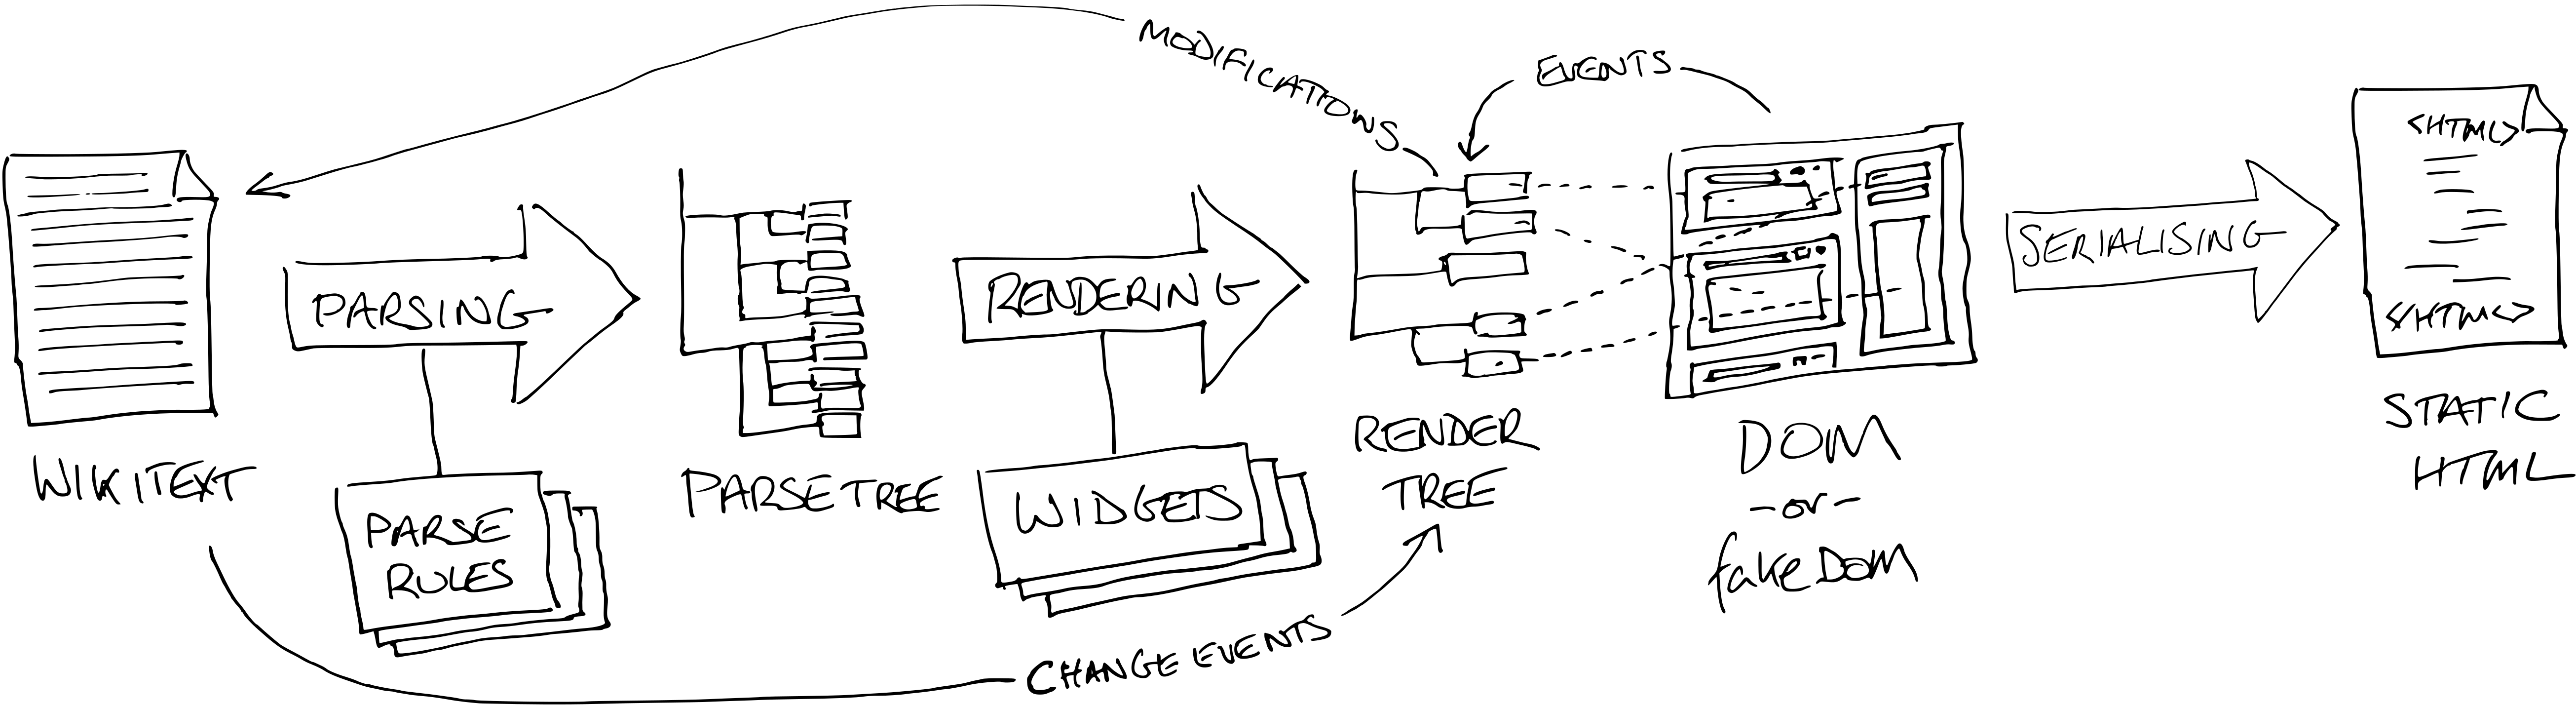
\includegraphics[scale=0.075]{images/TiddlyWikiArchitecture.png}
\end{figure}

\newpage
\subsection{Data Persistence 1-2}

\subsubsection*{Persist data}
TiddlyWiki supports a wide range of methods to persist your data. One of this methods is the HTML5 fallback saver. This methods works on almost every browser. With this method a copy of the entire wiki will be downloaded by the browser. This means you get a new file everytime you hit the save button.  To avoid this and because every Browser has a different API to allow writing direct to the file system there a some plugins for the different browsers. These plug-ins allow the user to save direct to the current open TiddlyWiki-File. The Listing below shows the HTML5-compliant to save the changes via the HTML5 fallback saver by downloading the TW as a complete HTML-file.
\begin{lstlisting}[caption={Download-Method of TW},label=lst:download]
DownloadSaver.prototype.save = function(text,method,callback) {
	...
	var link = document.createElement("a");
	link.setAttribute("target","_blank");
	...
	link.setAttribute("href","data:text/html," + encodeURIComponent(text));
	...
	link.setAttribute("download",filename);
	document.body.appendChild(link);
	link.click();
	document.body.removeChild(link);
	return true;
};
\end{lstlisting}
\newpage
\subsubsection*{Data-Storage}
TW has two approaches to save the user data. These approaches depends on way you use TW. either you use node.js as a server for TW its saves the tiddlers as plain text in different files or you use TW as standalone in a browser it persists the data within the HTML-File in two Div-Areas depending on whether the encryption of the TiddlyWiki is activated or not. If the TiddlyWiki is not encrypted the data is stored in the Div-Area called ``StoreArea''. Every created Tiddler is stored in a own Div-area with a few custom values. An example of a saved Tiddler is shown below (\prettyref{lst:data-div}). 
\begin{lstlisting}[caption={Data-Div},label=lst:data-div]
<div created="20140611153703343" modified="20140611153734589" tags="testTag" testfield="testvalue" title="TestTiddler" type="text/plain">
	<pre>testText</pre>
</div>
\end{lstlisting}
The Div-Area has the same attributes like the standard tillder fields, listed in  (\prettyref{list:TiddlerFields}), all attributes which are not in this list are parsed as a custom field. The only required attribute is the name attribute, all other attributes are optional.\\
With a activated encryption the data is stored in a special Div-Area called ``encryptedStoreArea''. TiddlyWiki uses the Standford JavaScript Crypto Libary\footnote{\url{http://bitwiseshiftleft.github.io/sjcl/}}. The encrypted Tiddlers are saved in a JSON string within this Div-Area.

\newpage
\section{Summary and Conclusion 1-2}
\bibliography{tiddly}
\bibliographystyle{alpha}
\end{document}
